\section{Własne funkcje krzyżowania i mutacji}

\subsection{Krzyżowanie}

\subsubsection{Funkcja testowa}
Testu algorytmu zostały wykonane dla funkcji wielomodalnej nr. 13 z biblioteki \textit{cec2013}.

\begin{figure}[H]
	\centering
	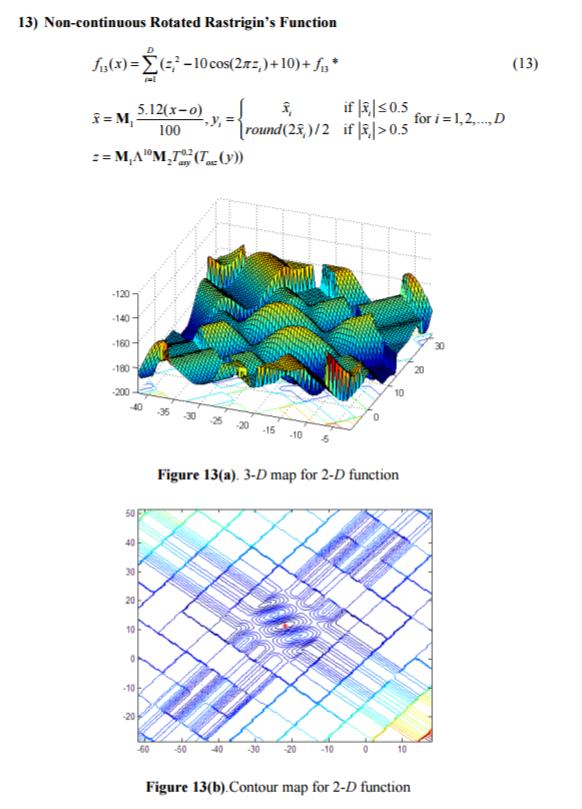
\includegraphics[scale=0.9]{f13}
	\caption{Funkcja testowa}
\end{figure}

W celu przetestowania możliwości użycia własnej funkcji krzyżowania zmodyfikowana została standardowa funkcja \textit{gareal\_waCrossover} z pakietu \textit{GA}.
Oryginalny współczynnik służący do określenia proporcji parametrów rodziców w potomstwie, określony przez rozkład jednostajny na zakresie (0-1) zastąpiony został wartością stałą, wynoszącą odpowiednio 0,6 i 0,4 dla rodziców. 

Wykonane zostały badania przy różnych wartościach parametru odpowiadającego za szansę mutacji oraz wielkości populacji. Do analizy wyników posłużyły wartość znalezionego minimum oraz liczba iteracji po których algorytm kończył działanie. Pozwala to analizować jednocześnie jakość wyniku i czas potrzebny na jego znalezienie - co w przypadku rzeczywistych zastosowań ma równie duże znaczenie.

Wszystkie przedstawione wyniki są uśrednieniem wyników z 30 uruchomień algorytmu, maksymalna ilość iteracji to 250, obszar poszukiwań minimum:

\begin{equation}
x\in [-60, 10] 
\nonumber
\end{equation}
\begin{equation}
y\in [-50, 20]
\nonumber
\end{equation}

Pozostałe parametry przyjmowały wartości domyślne dla pakietu \textit{GA}.
\subsubsection{Wyniki w zależności od prawdopodobieństwa krzyżowania}
\begin{figure}[H]
	\centering
	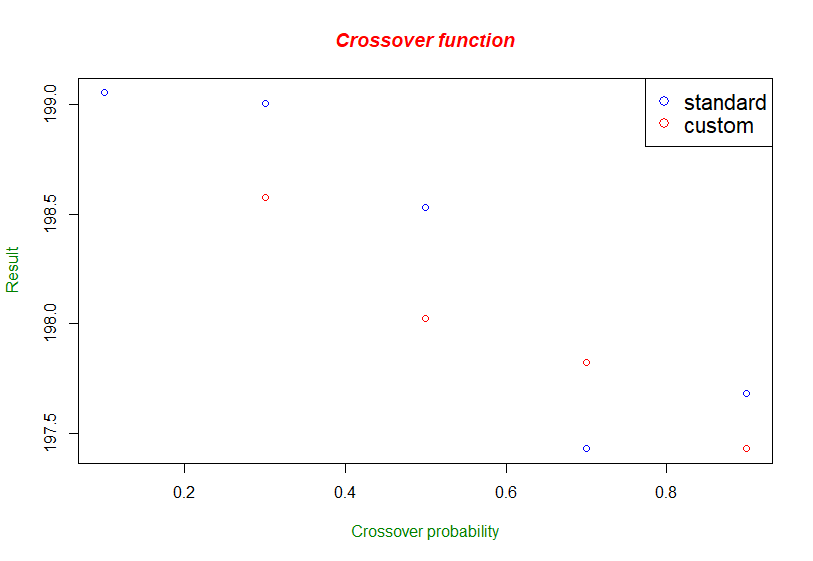
\includegraphics[scale=0.5]{custCrossover_pcross_result}
	\caption{Rezultat optymalizacji dla różnych wartościach prawdopodobieństwa krzyżowania}

\end{figure}

\begin{figure}[H]
	\centering
	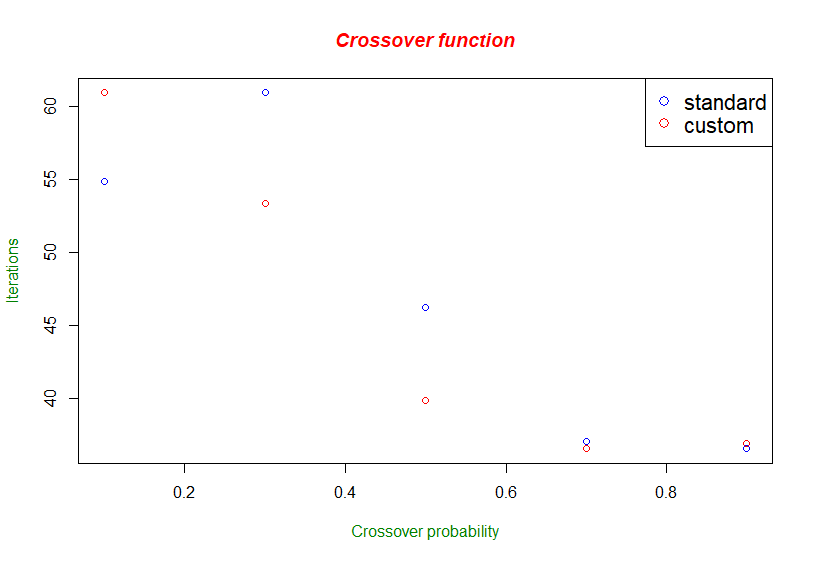
\includegraphics[scale=0.5]{custCrossover_pcross_iterations}
	\caption{Ilość iteracji dla różnych wartościach prawdopodobieństwa krzyżowania}
\end{figure}


\subsubsection{Wyniki w zależności od wielkości populacji}

\begin{figure}[H]
	\centering
	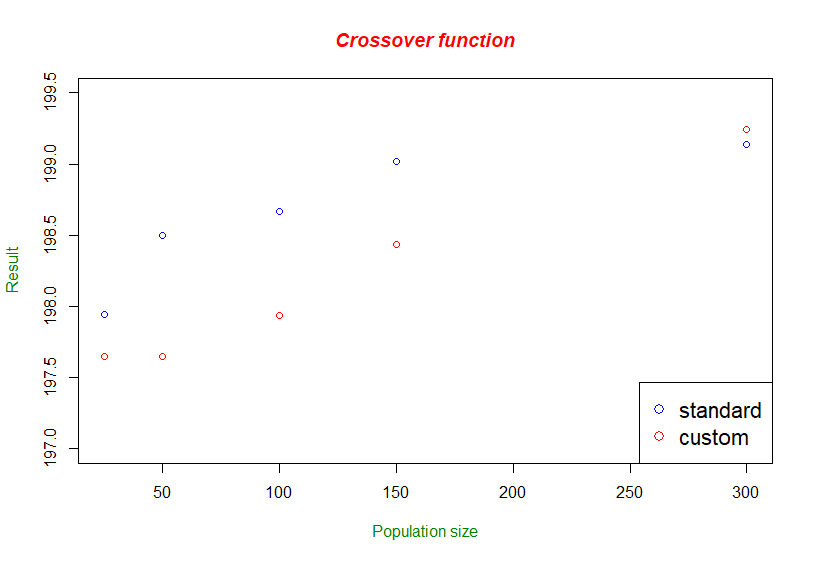
\includegraphics[scale=0.5]{custCrossover_popSize_results}
	\caption{Rezultat optymalizacji dla różnych wielkości populacji}

\end{figure}

\begin{figure}[H]
	\centering
	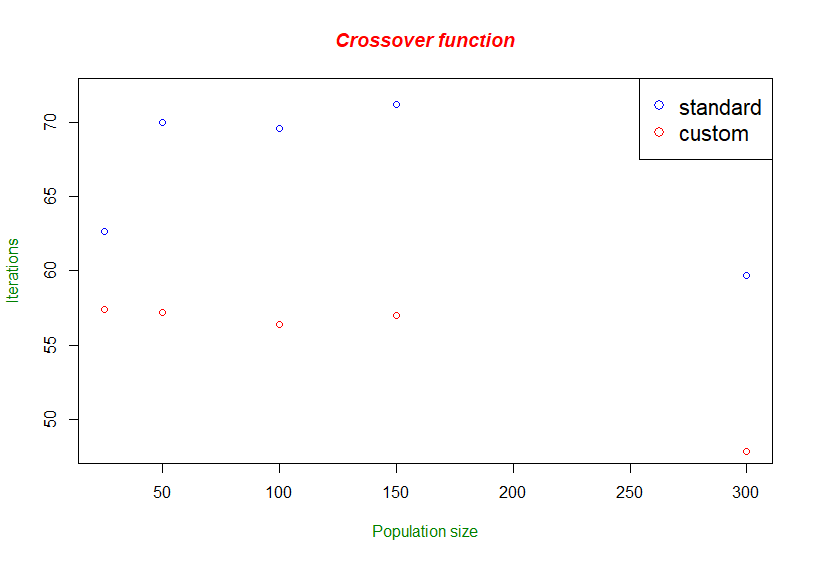
\includegraphics[scale=0.5]{custCrossover_popSize_iterations}
	\caption{Ilość iteracji dla różnych wielkości populacji}
\end{figure}

\subsubsection{Wnioski}

Modyfikacja algorytmu poprzez wyeliminowanie zmiennej losowej z funkcji krzyżowania spowodowała pogorszenie osiąganych przez algorytm genetyczny wyników. Algorytm genetyczny po modyfikacji krzyżowania słabiej odnajduje minimum w ramach pojedynczego minimum lokalnego co przedstawia się w mniejszej ilości iteracji wykonywanych przez algorytm - przy braku progresu funkcja stopu kończy działanie programu.

\subsection{Mutacja}